\section{Transistoren}
\subsection{Übersicht Transistoren}
  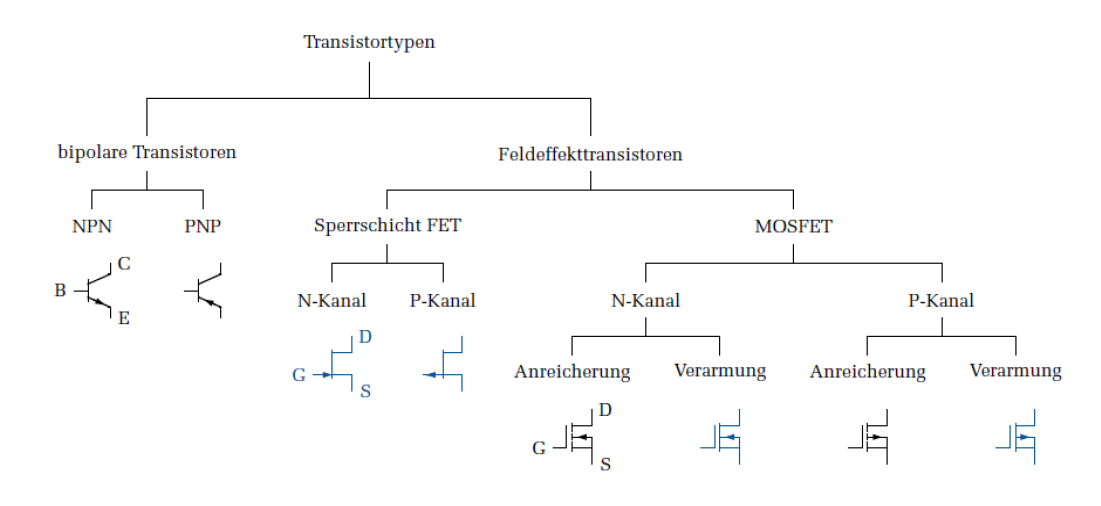
\includegraphics[width=12cm]{./bilder/transistoren_uebersicht.png}
\subsection{Bipolar-Transistor}
  \subsubsection{Ebers-Moll-Ersatzschaltbild}
    \begin{minipage}[T]{16cm}
      Kollektorstrom
      \hspace{18.7mm}\fbox{$I_C = A_N\cdot I_{ES} \cdot\left(e^{\frac{U_{BE}}{U_T}}-1\right) - I_{CS}\cdot\left( e^{\frac{U_{BC}}{U_T}}-1\right)       = A_N \cdot I_{ED} - I_{CD}$}\\
      Emitterrstrom
      \hspace{19.7mm}\fbox{$I_E = I_{ES} \cdot\left(e^{\frac{U_{BE}}{U_T}}-1\right) - A_I\cdot I_{CS}\cdot\left( e^{\frac{U_{BC}}{U_T}}-1\right)      = I_{ED} - A_N \cdot I_{CD}$}\\
    \end{minipage}
    
    \begin{minipage}[T]{13cm}
      Basisstrom
      \hspace{25.1mm}\fbox{$I_B = I_E - I_C$}\vspace{1mm}\\ 
      \hspace*{43mm}$I_{ES}/I_{CS}$: S\"attigungssperrstrom von Emitter/Kollektor\\
      \hspace*{43mm}$U_T$: Thermospannung\\
      \hspace*{43mm}$A_N / A_I$: Verst\"arkungsfaktoren\\
      \hspace*{43mm}$I_{ED}/I_{CD}$: Diodenvorw\"artsstr\"ome (siehe Diode)\\
    \end{minipage}
    \begin{minipage}[T]{6cm}
      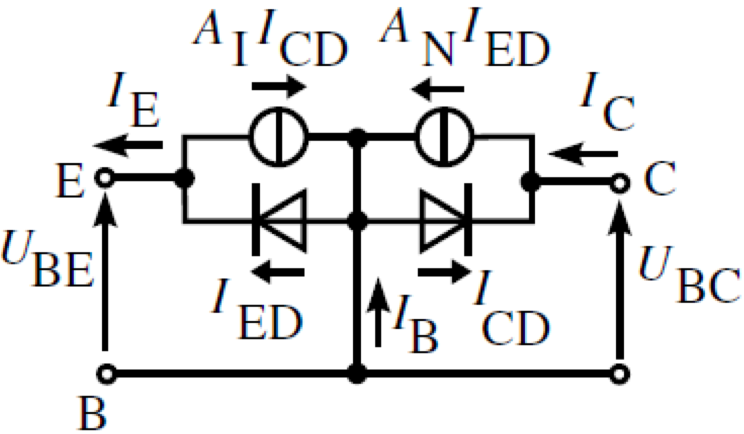
\includegraphics[width=6cm]{./bilder/EberMollModell.png}
    \end{minipage}
            
  \subsubsection{Stromverst\"arkungsfaktoren}
    \begin{minipage}[T]{6cm}
      \bf Basisschaltung\\
      \fbox{$A_N = \frac{I_C}{I_E}$}\\
      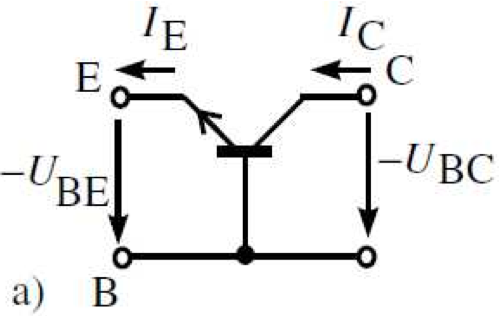
\includegraphics[height=2.3cm]{./bilder/AmpBasisSch.png}
    \end{minipage}
    \begin{minipage}[T]{6cm}
      \bf Emitterschaltung\\
      \fbox{$B_N = \frac{I_C}{I_B} = \frac{A_N}{1-A_N}$}\\
      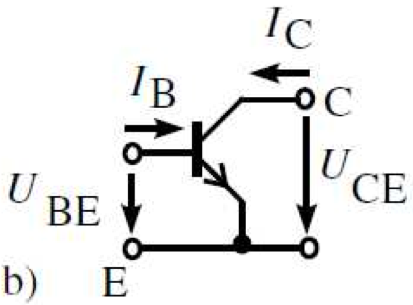
\includegraphics[height=2.3cm]{./bilder/AmpEmitSch.png}                
    \end{minipage}
    \begin{minipage}[T]{6cm}
      \bf Kollektorschaltung\\
      \fbox{$C_N = \frac{I_E}{I_B} = \frac{1}{1-A_N}$}\\
      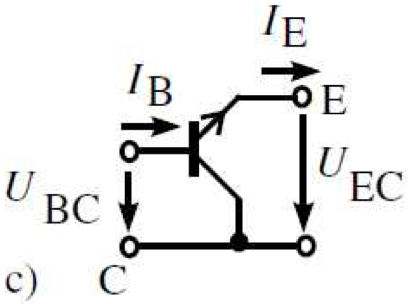
\includegraphics[height=2.3cm]{./bilder/AmpKolSch.png}                
    \end{minipage}
    
\hrule

  \subsubsection{Kennlinienfelder}
    \begin{minipage}[T]{14cm}
      {\bf Ausgangskennlinie (I) $I_C(V_{CE})$}\\
      typ.: $V_{CE_{sat}}=0.3V$ und Ausgangswiderstand \fbox{$r_{CE} \cong \frac{V_{Early}}{I_{C0}}$}\\
      mit berücksichtigung des Early-Effekts gilt 
      \fbox{$I_C = (B_N\cdot I_B + I_{CE0})\left(1+\frac{U_{CE}}{U_{Early}}\right)$}
      \hrule\vspace{1mm}
      {\bf Strom\"ubertragungskennlinie (II) $I_C(I_B)$}\\
      Kollektorstrom: $I_C = \frac{A_N}{1-A_N}\cdot I_B + \frac{A_N\cdot (1-A_I)}{1-A_N}\cdot I_{CS} = B_N\cdot I_B + I_{CE0} \cong B_N\cdot I_B$\\
      \hrule\vspace{1mm}
      {\bf Eingangskennlinie (III)}\\
      Basisstrom: $I_B = I_{ES}\cdot\left(e^{\frac{V_{BE}}{V_T}}-1\right)$\\
      Kleinsignalwiderstand: \fbox{$r_{BE} = \frac{m\cdot V_T}{I_{B0}} = \frac{dV_{BE}}{dI_B}$} mit $I_{B0}$: Arbeitspunktstrom\\
      \hrule\vspace{1mm}
      {\bf Spannungsr\"uckwirkungskennlinie (IV)}\\
      $V_{BE} = \eta \cdot V_{CE}$ mit $\eta \cong 0.1 \%$ (kann meist vernachl\"assigt werden!)\\
    \end{minipage}
    \begin{minipage}[T]{5cm}
      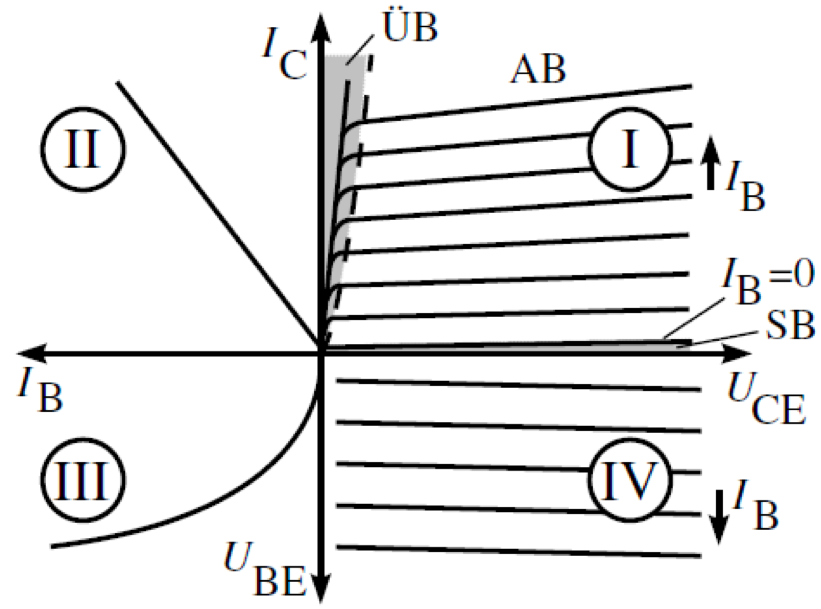
\includegraphics[width=5cm]{./bilder/BipTraKennlinien.png}\\
      ÜB: Übersteuerungsbereich\\
      AB: Arbeitsbereich\\
      SB: Sperrbereich
    \end{minipage}
    


  \subsubsection{Kleinsignal-Modell}
    \begin{minipage}[T]{14cm}
      \begin{tabular}{p{3.5cm} l}
        Eingangswiderstand & 
        \fbox{$r_B =h_{11e} = \left.\frac{dU_{BE}}{dI_B}\right|_{U_{CE0}} = \frac{U_T}{I_{B0}} $}\\
     
        Spannungsrückwirkung & 
        \fbox{$\eta=h_{12e} = \left.\frac{dU_{BE}}{dU_{CE}}\right|_{I_{B0}} \approx 0$}\\
        %
        Stromverst\"arkung & 
        \fbox{$b = h_{FE} = \left.\frac{IC}{I_B}\right|_{U_{CE0}} =B_N\cdot\left(1+\frac{U_{CE0}}{U_{Early}}\right) \approx B_N$}\\
        %
        Ausgangswiderstand &
        \fbox{$r_{CE} = \left.\frac{dU_{CE}}{dI_C}\right|_{I_{B0}} \cong \frac{U_{EA}}{I_{C0}}$}\\
        
        Steilheit &
        \fbox{$S = \frac{b}{r_{BE}} = \frac{I_{C0}}{m\cdot V_T} = g_m = \frac{dI_{OUT}}{dV_{IN}}$}\\
        
        
      \end{tabular}
    \end{minipage}
    \begin{minipage}[T]{5cm}
      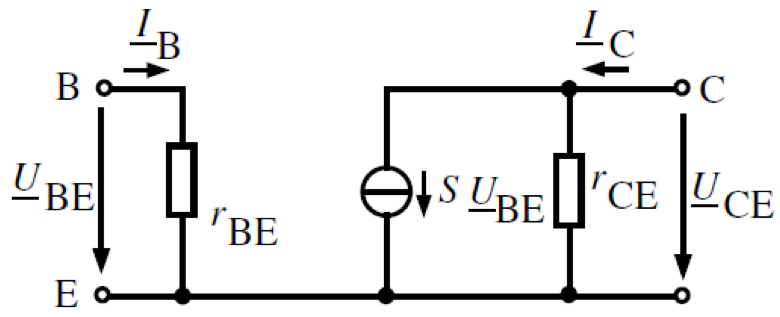
\includegraphics[width=5cm]{./bilder/BipTraErsatzsch.png}\\
      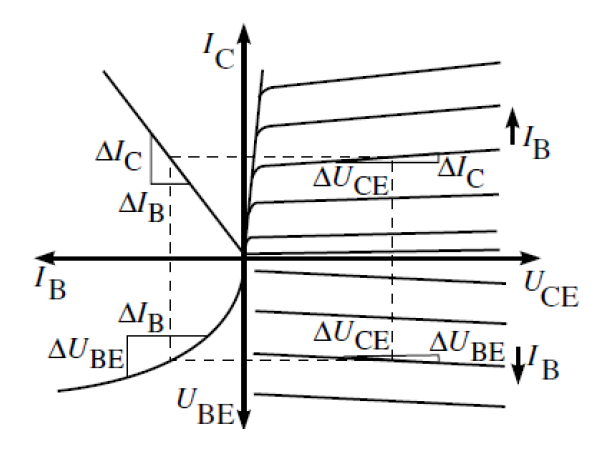
\includegraphics[width=5cm]{./bilder/KleinSigMod.png}
    \end{minipage}
            
  \subsubsection{Kleinsignal-Ersatzschaltung der Emitterschaltung}
    \begin{minipage}[T]{14cm}
      Ausgangsspannung
      \hspace{13mm}\fbox{$U_a = -b\cdot I_B\cdot(R_C // r_{CE})$}\\
      Basisstrom
      \hspace{25.3mm}\fbox{$I_B = \frac{U_e}{r_{BE}}$}\\
      Verst\"arkung
      \hspace{23.3mm}\fbox{$V_U = \frac{U_a}{U_e} = -\frac{b}{r_{BE}}\cdot(R_C//r_{CE}) = -S\cdot(R_C//r_{CE})$}\\
    \end{minipage}
    \begin{minipage}[T]{5cm}
      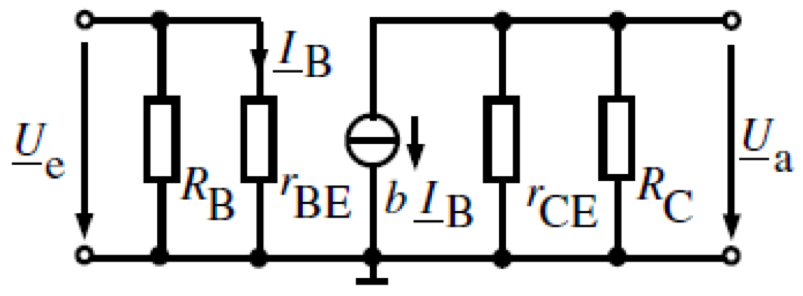
\includegraphics[width=5cm]{./bilder/KleinSigErsEmmitersch.png}
    \end{minipage}
            
    \subsubsection{Frequenzabh\"angigkeit des Bipolartransistors}
      \begin{minipage}[T]{11cm}
        Stromverst\"arkung
        \hspace{14.5mm}\fbox{$h_{21e}(\omega)\approx \frac{b}{1+ \jmath\omega\cdot r_{BE}\cdot (C_E + C_{BE)}}$}\\
        bei $\omega$ = Transitfrequenz $\omega_T$ ist die Stromverst\"arkung $h_{21e} = 1$\\
        Transitfrequenz wird ebenfalls als Gain-Bandwith-Product GBP\\bezeichnet.
        $\omega_1 = \omega_T = b\cdot \omega_{\beta} \approx \omega_{\alpha}$
      \end{minipage}
      \begin{minipage}[T]{8cm}
        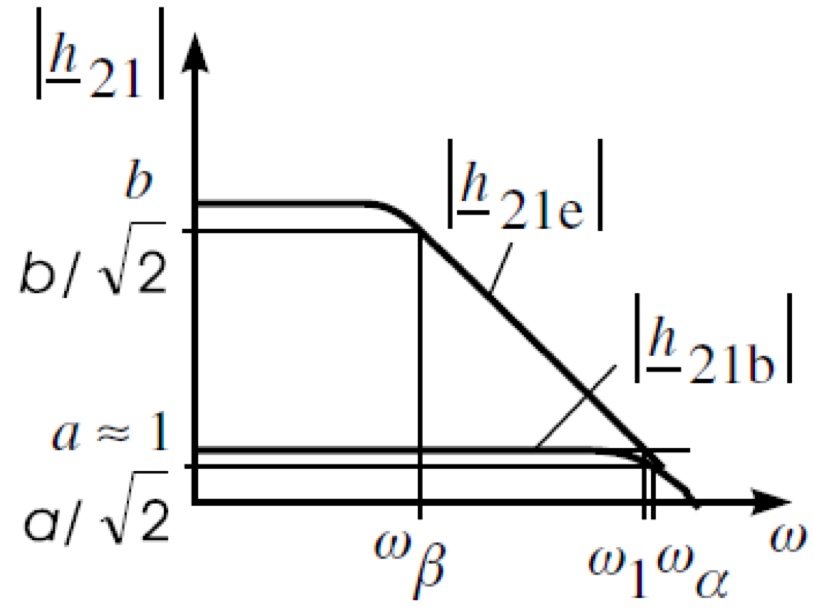
\includegraphics[width=3cm]{./bilder/BipTraFrequenzgang.png}
        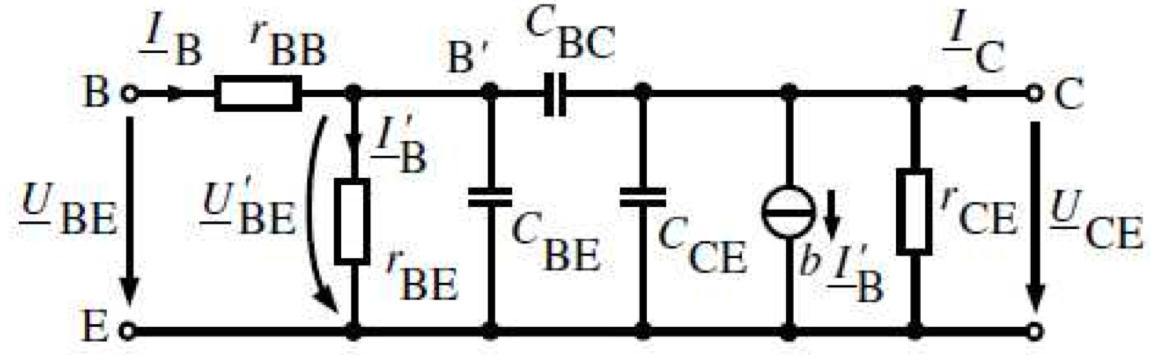
\includegraphics[width=5cm]{./bilder/BipTraErsatzschFreq.png}
      \end{minipage}
            
  \subsubsection{Temperaturverhalten von Bipolartransistoren}
    Temperaturabhängigkeit von $V_{BE}: -2mV/K$ und somit Verdoppelung des Sperrstromes bei Temperaturerh\"ohung um $10K$\\
    \begin{tabular}{ll}
      Stromverst\"arkungsfaktor &
      \fbox{$B_N(T) = B_N(T_0)\cdot e^{C_b\cdot(T-T_0)}$ mit $C_b \approx 0.6\% \cdot K^{-1}$}\\
      
      Thermischer Widerstand &
      \fbox{$P_{Vmax} = \frac{T_{max} - T_U}{R_{th}}$} \newline
      mit $R_{th} = 0.25K/mW \rightarrow$ für TO-92 Plastikgehäuse \\
    \end{tabular}
    \vspace{2mm}\hrule
    
  

  \subsubsection{Transistor als Schalter}
    \begin{minipage}[T]{13cm}
      Bei der Verwendung des Transistors als Schalter berechnet man den Basisstrom aufgrund des erforderlichen Kollektorstromes und dem           
      vorhandenen Stromverst\"arkungsfaktor und vergr\"ossert den Basisstrom dann anschliessend noch um den Faktor 2 bis 5. Dadurch wird    
      erreicht, dass der Transistor auf jeden Fall v\"ollig durchgeschaltet wird.
    \end{minipage}
    \begin{minipage}[T]{6cm}
      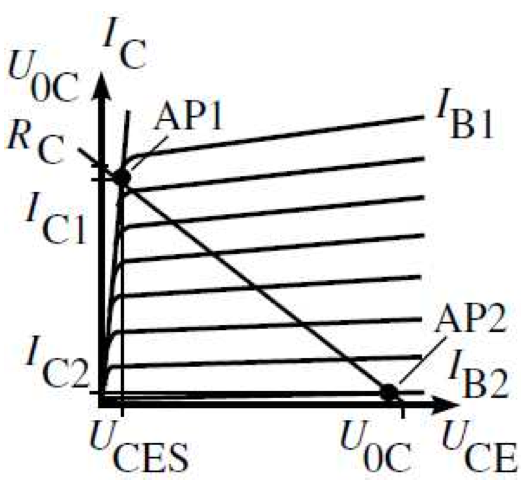
\includegraphics[height=3cm]{./bilder/BipTrAlsSchalterKennl.png}
      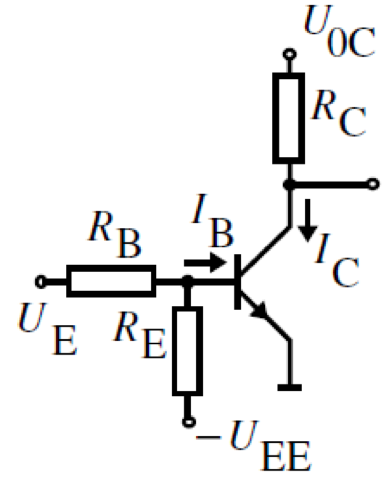
\includegraphics[height=3cm]{./bilder/BipTrAlsSchalter.png}
    \end{minipage}
            
  \subsubsection{Gegenkopplungsschaltungen zur Reduktion der Abh\"angigkeit von Temperatur und Tolleranzen}
    \begin{minipage}[T]{5.4cm}
      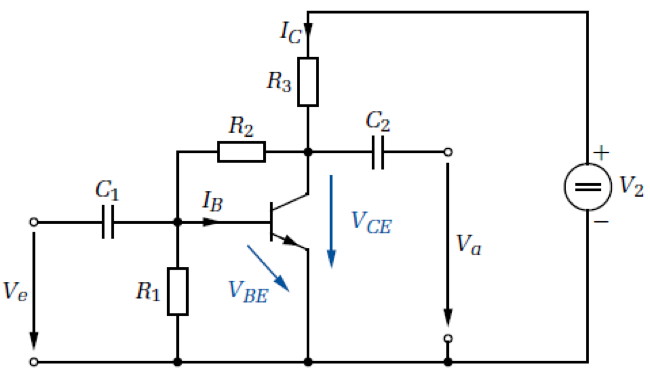
\includegraphics[height=3cm]{./bilder/Spannungsgegenkopplung.png}\\
      Spannungsgegenkopplung
    \end{minipage}
    \begin{minipage}[T]{4cm}
      Gegenkopplung durch $R_2$
    \end{minipage}
    \vrule \hspace{0.1cm}
    \begin{minipage}[T]{5.5cm}
      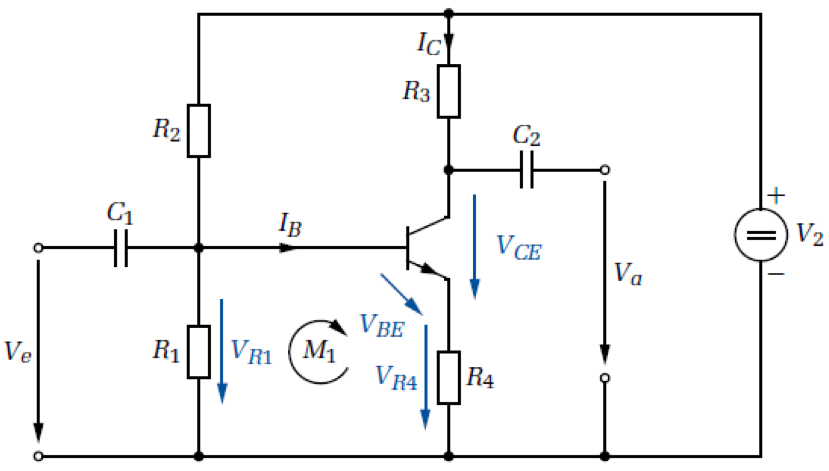
\includegraphics[height=3cm]{./bilder/Stromgegenkopplung.png} \\
      Stromgegenkopplung
    \end{minipage}
    \begin{minipage}[T]{4cm}
      Gegenkopplung durch $R_4$\\\\
      $V_{out} = -\frac{R_3}{R_4}\cdot V_{in}$\\\\
      Verst\"arkung viel kleiner als ohne Gegenkopplung
    \end{minipage}
            
  \subsubsection{Transistorverst\"arkerschaltungen}
    \begin{minipage}[T]{4.7cm}
      Emitterschaltung mit\\
      Stromgegenkopplung\\
      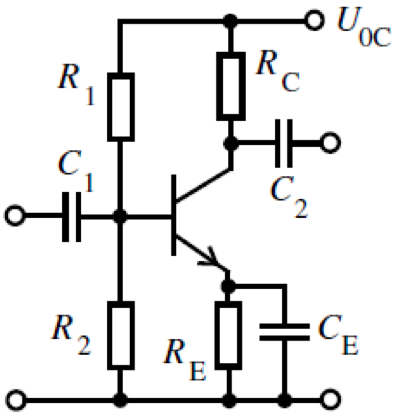
\includegraphics[height=3cm]{./bilder/BipTraEmitterschStGk.png}
    \end{minipage}
    \begin{minipage}[T]{4.7cm}
      Emitterschaltung mit\\
      Spannungsgegenkopplung\\
      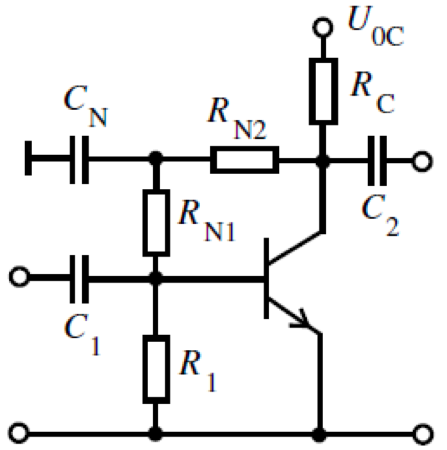
\includegraphics[height=3cm]{./bilder/BipTraEmitterschSpGk.png}
    \end{minipage}
    \begin{minipage}[T]{5.7cm}
      Basisschaltung\\
      (Impedanzwandler)\\
      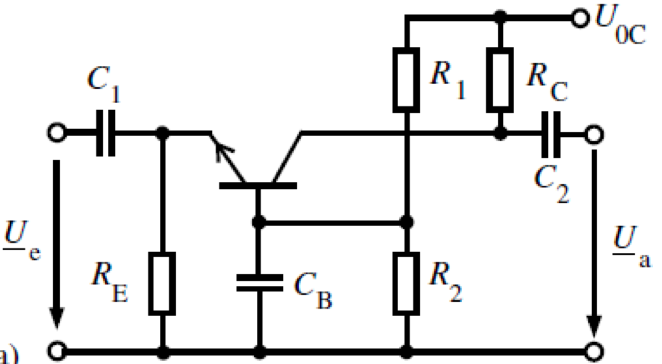
\includegraphics[height=3cm]{./bilder/BipTraBasissch.png}
    \end{minipage}
    \begin{minipage}[T]{3.7cm}
      Kollektorschaltung\\
      (Emitterfolger)\\
      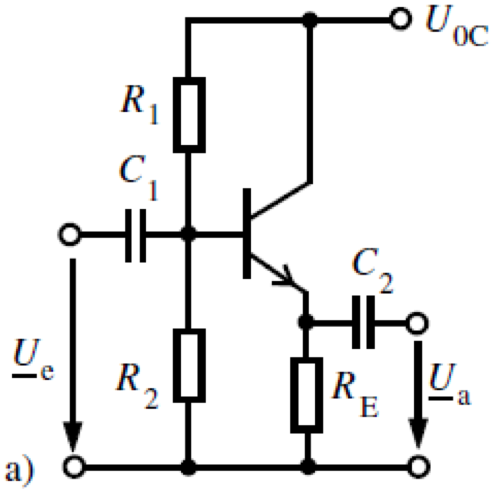
\includegraphics[height=3cm]{./bilder/BipTraKollektorsch.png}
    \end{minipage}
    

  \subsection{Stromspiegel}
    \begin{minipage}{9cm}
      Spiegelverhältnis \fbox{$M = \frac{b}{b+2} = 1-\frac{2}{b+2} \approx 1$} \\
      Er spiegelt einen Referenzstrom wieder. Bei grosser Stromverstärkung ist das
      Spiegelverhältnis annähernd 1.
    \end{minipage}
    \begin{minipage}{9cm}
      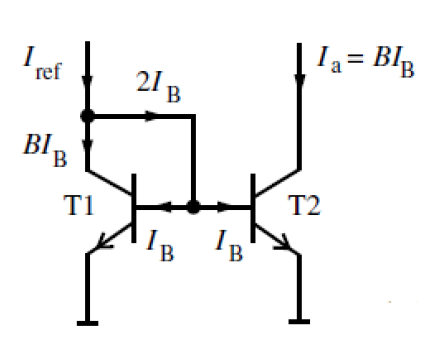
\includegraphics[width=6cm]{./bilder/Stromspiegel.png}
    \end{minipage}

  \subsubsection{Differenzverst\"arker}
    \begin{minipage}[T]{11cm}
      Differenz-Verst\"arkung
      \hspace{8.4mm}\fbox{$v_d = \frac{U_{A_d}}{U_{E_d}} = -S \cdot (R_C//r_{CE}) \approx -S\cdot R_C$}\\
      Gleichtaktverst\"arkung
      \hspace{8.1mm}\fbox{$v_{gl} = -\frac{R_C}{2\cdot R_E}$}\\
      Gleichtaktunterdr\"uckung
      \hspace{3.8mm}\fbox{$G = \frac{v_d}{v_{gl}} = 2\cdot S \cdot R_E$}\\
      Ausgangsstrom
      \hspace{18.8mm}\fbox{$I_{out} = gm \cdot (V_{e1} - V_{e2})$} \\
      Transkonduktanz
      \hspace{15.6mm}\fbox{$gm = \frac{dI_{out}}{dU_{in}}$} \\
      Transimpedanz
      \hspace{19mm}\fbox{$\frac{dU_{out}}{dI_{in}}$}
    \end{minipage}
    \begin{minipage}[T]{4cm}
      S = Steilheit \\
      $U_{Ad}$ = Ausgangsdifferenz \\
      $U_{Ed}$ = Eingangsdifferenz \\
    \end{minipage}
    \begin{minipage}{4cm}
      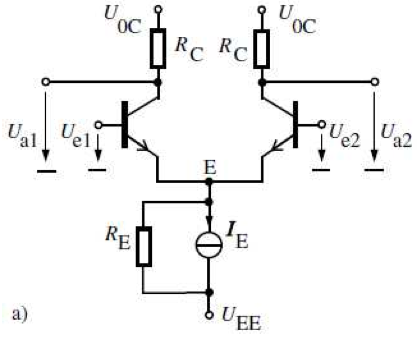
\includegraphics[height=3cm]{./bilder/BipTraDiffAmp.png}
    \end{minipage}\\
             
    \subsubsection{Leistungsendstufen}
      \begin{minipage}[T]{4.7cm}
        Klasse A-Verst\"arker\\
        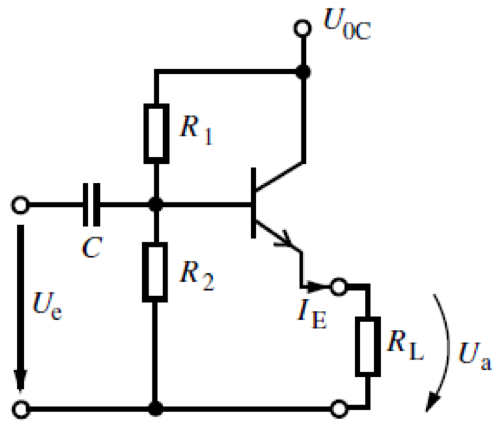
\includegraphics[height=4cm]{./bilder/KlassA_Amp.png}\\
        $\eta_{max} = \frac{P_{\sim max}}{P_=} = 25\%$
      \end{minipage}
      \begin{minipage}[T]{4.7cm}
        Klasse B-Verst\"arker\\
        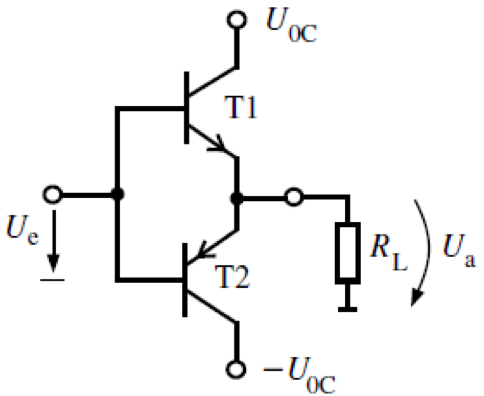
\includegraphics[height=4cm]{./bilder/KlassB_Amp.png} \\
        $\eta_{max} = \frac{P_{\sim max}}{P_=} = 78.5\%$
      \end{minipage}
      \begin{minipage}[T]{4.7cm}
        Klasse AB-Verst\"arker\\
        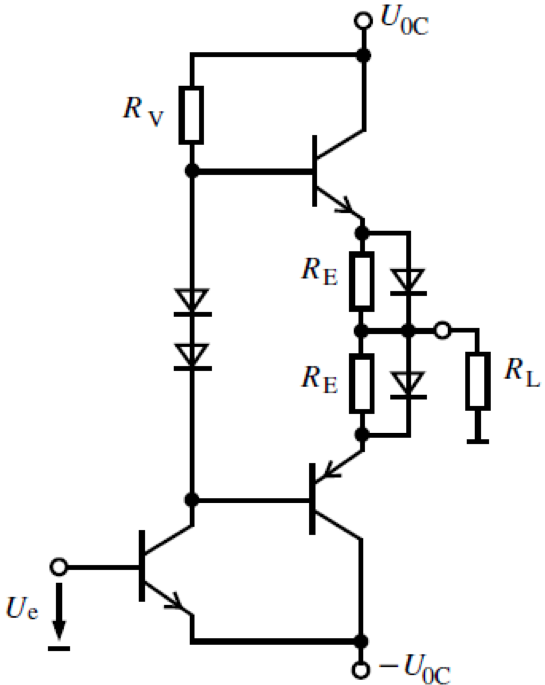
\includegraphics[height=4cm]{./bilder/KlassAB_Amp.png}
      \end{minipage}
      \begin{minipage}[T]{4.7cm}
        Arbeitspunkte jeweiler Klassen\\\\
        \vspace{5mm}
        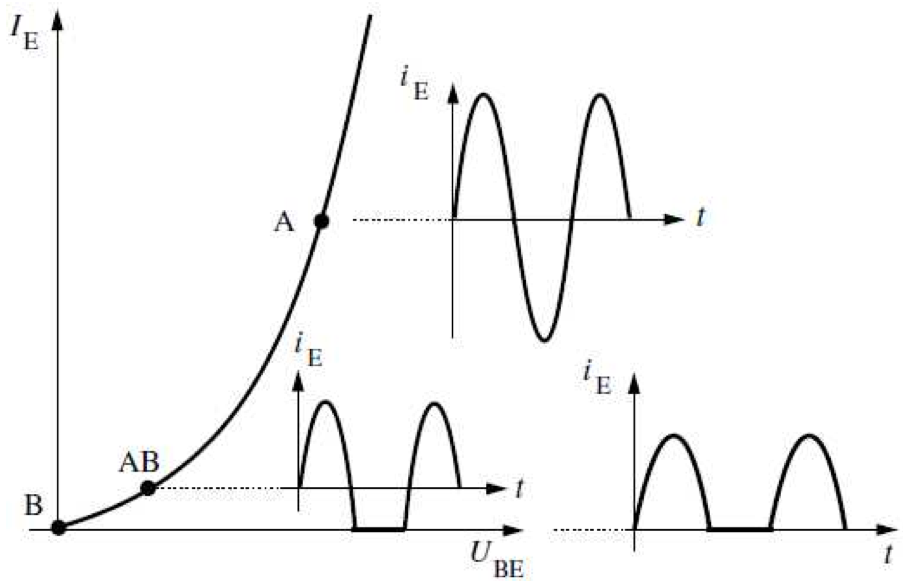
\includegraphics[width=4.7cm]{./bilder/EndstufenAP.png}
      \end{minipage}
      
\vspace{2mm}\hrule

\subsection{FET-Transistor}
  \subsubsection{JFET Junction Field Effect Transistor}
    \begin{minipage}[T]{8cm}
      JFET als {\bf Konstantstromquelle}:\\
      ben\"otigter Strom \fbox{$I_D = \frac{U_{GS}}{R_S}$}\\
      $U_{GS}$ entsprechend ben\"otigem Strom aus Kennlinie lesen\\
      bei der Pinch-off-Grenze (Abschn\"urgrenze) sperrt der JFET
    \end{minipage}
    \begin{minipage}[T]{3.4cm}
      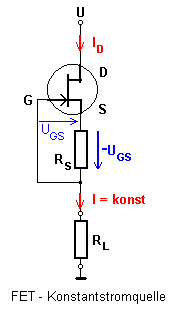
\includegraphics[height=4cm]{./bilder/JFETCCQuelle.png}
    \end{minipage}
    \begin{minipage}[T]{6cm}
      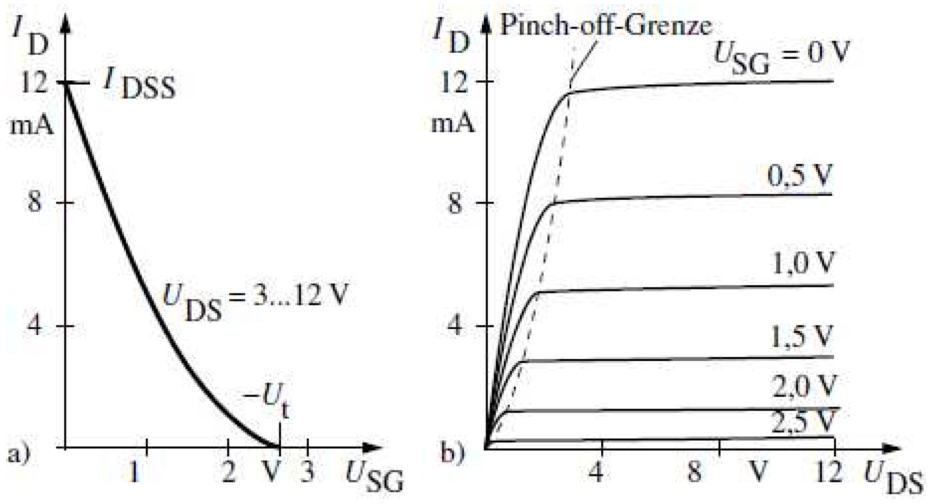
\includegraphics[height=4cm]{./bilder/JFETKennlinie.png}
    \end{minipage}
    
\hrule

  \subsubsection{MOSFET Metal Oxide Silicon Field Effect Transistor}
    Thermisches Verhalten $\frac{dU_T}{dT} \approx -1 mV/K$ \\
    \begin{minipage}[T]{6cm}
      \underline{Sperrbereich}\\\\
      $V_{GS} < V_{th} \to I_D = 0$\\
      typische $V_{th} = 0.5 \ldots 1.5V$\\ 
      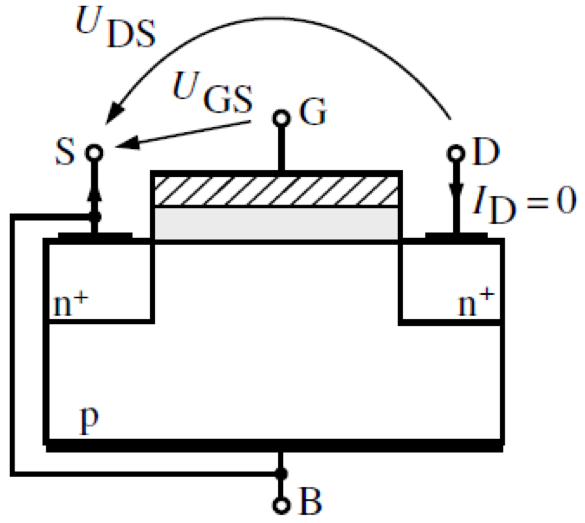
\includegraphics[height=4cm]{./bilder/MOSFETSperrbereich.png}
    \end{minipage}
    \begin{minipage}[T]{6cm}
      \underline{Widerstands-/Triodenbereich (linear)}\\\\
      $V_{GS} > V_{th} $ und $0 < V_{DS} \leq V_{GS} - V_{th}$\\
      $\to I_D$ fliesst\\
      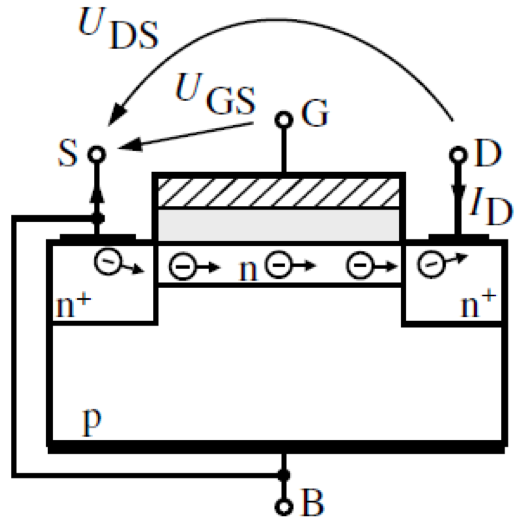
\includegraphics[height=4cm]{./bilder/MOSFETLinBereich.png}
    \end{minipage}
    \begin{minipage}[T]{6cm}
      \underline{S\"attigungs-/Pentodenbereich}\\\\
      $0 < V_{GS} - V_{th} \leq V_{DS}$, mit $V_{GS} > V_{th}$ Kanal wird abgeschn\"urt\\
      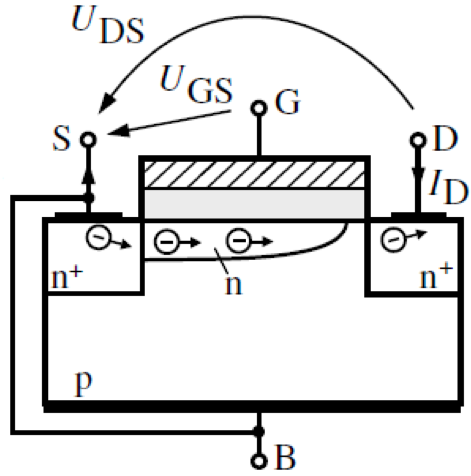
\includegraphics[height=4cm]{./bilder/MOSFETSaettBereich.png}
    \end{minipage}\\
            
  \subsubsection{Steuerkennlinien von verschiedenen MOSFETs}
    \begin{minipage}[T]{9cm}
      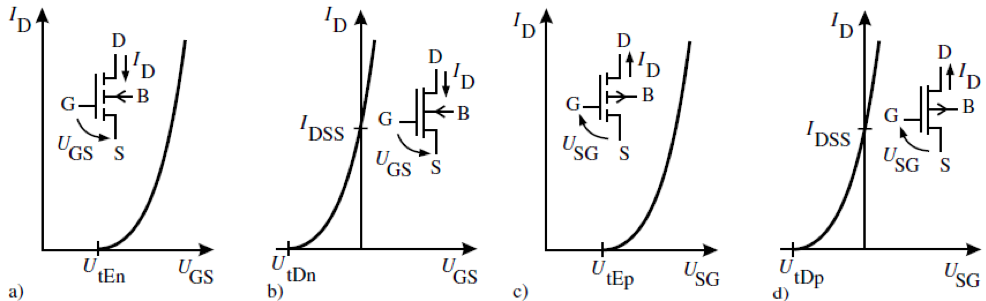
\includegraphics[height=2.4cm]{./bilder/MOSFETSteuerkennlinien.png}
    \end{minipage}
    \begin{minipage}[T]{9cm}
      a) n-Kanal Anreicherungs-Typ (selbstsperrend)\\
      b) n-Kanal Verarmungs-Typ (selbstleitend)\\
      c) p-Kanal Anreicherungs-Typ (selbstsperrend)\\
      d) p-Kanal Verarmungs-Typ (selbstleitend)\\
    \end{minipage}
                
  
      
  \subsubsection{Berechnung des Drainstromes $I_D$}
    \begin{minipage}{13cm}
      $I_D = \begin{cases}
        0 & $f\"ur $ V_{GS} \leq V_{th}\\
        {\bf Sperrbereich}\\\\
        
        \beta\cdot(2(V_{GS}-V_{th})V_{DS} - V_{DS}^2)\cdot(1 + \lambda\cdot V_{DS}) &  $f\"ur $ 0 < V_{DS} \leq V_{GS}-V_{th},\\
        {\bf Triodenbereich} $ TB linearer Bereich$ & V_{GS} > V_{th}\\ \\
        
        \beta\cdot(V_{GS} - V_{th})^2\cdot(1 + \lambda\cdot V_{DS})    &  $f\"ur $ 0\leq V_{GS} - V_{th} \leqq V_{DS}\\
        {\bf Pentodenbereich} $ PB S\"attigungsbereich $\\
      \end{cases}$\\
                
      \begin{tabular}[t]{l l l}
        $b$: Kanalbreite & $L$: Kanall\"ange & $\mu_n$: Leitf\"ahigkeit Kanal\\
        $\epsilon_{ox}$: Dielektrizit\"at Oxidschicht & $\lambda$: Pinch-off-Konstante & $d_{ox}$: Oxiddicke\\
        $V_{th}$: Threshold-Spannung & $\beta$: Steilheitsparameter & $K$: Steilheitskoeffizient
      \end{tabular}
    \end{minipage}
    \vrule \hspace{0.1cm}
    \begin{minipage}[T]{6cm}
      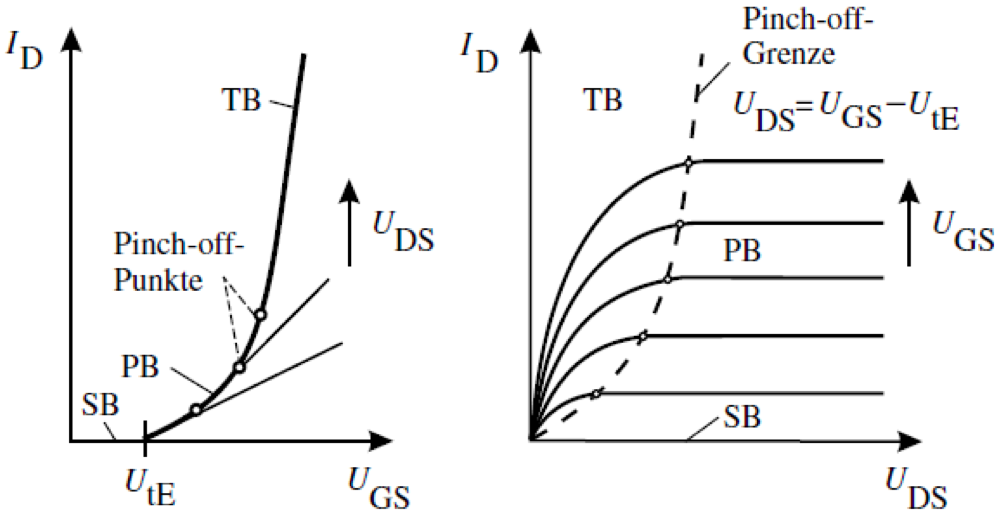
\includegraphics[width=6cm]{./bilder/MOSFET_IU_Kennlinie.png}\\
      \vspace{0.8cm}\\
      Steilheitsparameter \hspace{1mm}\fbox{$\beta = \frac{K}{2} = \frac{\mu_n \epsilon_{ox}}{2d_{ox}}\frac{b}{L}$}
    \end{minipage}\\
            
  \subsubsection{Kleinsignalmodell des MOSFET}
    \begin{minipage}[T]{10.5cm}
      Steilheit
      \hspace{29.3mm}\fbox{$g_m = 2\beta(V_{GS}-V_{th}) = \sqrt{4\beta\cdot I_D}$}\\
      Ausgangsleitwert
      \hspace{15.9mm}\fbox{$g_d = \beta\lambda(V_{GS}-V_{th})^2$}\\
      Drain-Source-Widerstand
      \hspace{3mm}\fbox{$r_{DS} = \frac{1}{\lambda\cdot I_{D0}}$}\\
      Gate-Source-Spannung
      \hspace{7mm}\fbox{$V_{GS} \cong \sqrt{\frac{I_D}{\beta}} + V_{th}$}
    \end{minipage}
    \begin{minipage}[T]{3.5cm}
      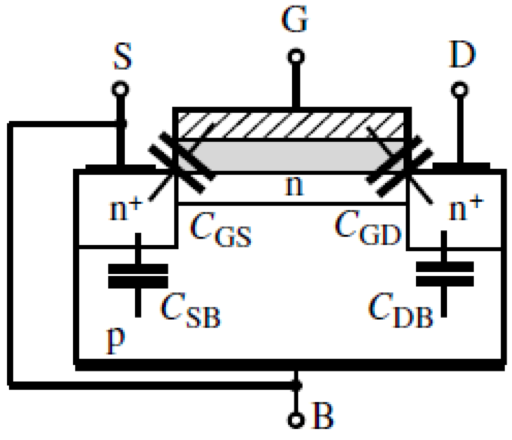
\includegraphics[width=3cm]{./bilder/MOSFET_Aufbau.png}
    \end{minipage}
    \begin{minipage}[T]{5cm}
      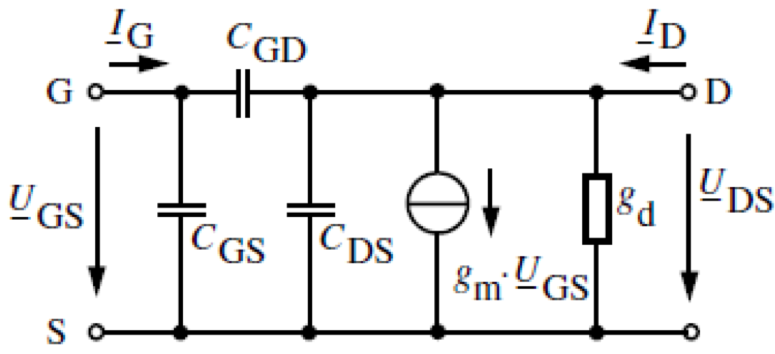
\includegraphics[width=5cm]{./bilder/MOSFET_Ersatzsch.png}
    \end{minipage}
    
\vspace{1mm}\hrule

  \subsubsection{Differenzverst\"arker}
    \begin{minipage}[T]{14cm}
      Ausgangswiderstand
      \hspace{10.6mm}\fbox{$r_{out} = R//r_{DS}$}\\
      Verst\"arkung
      \hspace{23.3mm}\fbox{$A_D = -S \cdot (R_D//r_{DS}) \approx -S \cdot R_D$}\\
      Ausgansdifferenzspannung
      \hspace{1.7mm}\fbox{$V_{A} = A \cdot V_{D}$}
                
    \end{minipage}
    \begin{minipage}[T]{5cm}
      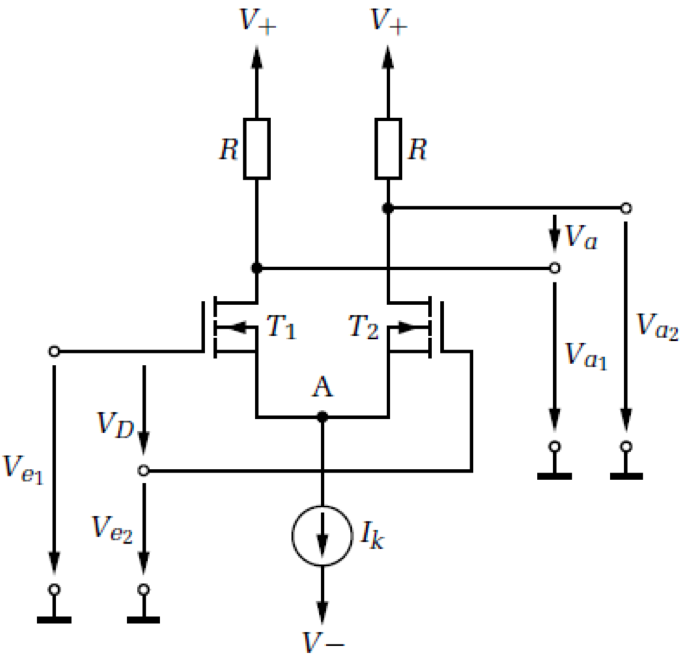
\includegraphics[height=4cm]{./bilder/MOSFET_Diffamp.png}
    \end{minipage}